%%
%% Copyright 2022 OXFORD UNIVERSITY PRESS
%%
%% This file is part of the 'oup-authoring-template Bundle'.
%% ---------------------------------------------
%%
%% It may be distributed under the conditions of the LaTeX Project Public
%% License, either version 1.2 of this license or (at your option) any
%% later version.  The latest version of this license is in
%%    http://www.latex-project.org/lppl.txt
%% and version 1.2 or later is part of all distributions of LaTeX
%% version 1999/12/01 or later.
%%
%% The list of all files belonging to the 'oup-authoring-template Bundle' is
%% given in the file `manifest.txt'.
%%
%% Template article for OXFORD UNIVERSITY PRESS's document class `oup-authoring-template'
%% with bibliographic references
%%

%%%CONTEMPORARY%%%
\documentclass[unnumsec,webpdf,contemporary,large]{oup-authoring-template}%
%\documentclass[unnumsec,webpdf,contemporary,large,namedate]{oup-authoring-template}% uncomment this line for author year citations and comment the above
%\documentclass[unnumsec,webpdf,contemporary,medium]{oup-authoring-template}
%\documentclass[unnumsec,webpdf,contemporary,small]{oup-authoring-template}

%%%MODERN%%%
%\documentclass[unnumsec,webpdf,modern,large]{oup-authoring-template}
%\documentclass[unnumsec,webpdf,modern,large,namedate]{oup-authoring-template}% uncomment this line for author year citations and comment the above
%\documentclass[unnumsec,webpdf,modern,medium]{oup-authoring-template}
%\documentclass[unnumsec,webpdf,modern,small]{oup-authoring-template}

%%%TRADITIONAL%%%
%\documentclass[unnumsec,webpdf,traditional,large]{oup-authoring-template}
%\documentclass[unnumsec,webpdf,traditional,large,namedate]{oup-authoring-template}% uncomment this line for author year citations and comment the above
%\documentclass[unnumsec,namedate,webpdf,traditional,medium]{oup-authoring-template}
%\documentclass[namedate,webpdf,traditional,small]{oup-authoring-template}

%\onecolumn % for one column layouts

%\usepackage{showframe}

\graphicspath{{main-figures/}}

% line numbers
%\usepackage[mathlines, switch]{lineno}
%\usepackage[right]{lineno}

\theoremstyle{thmstyleone}%
\newtheorem{theorem}{Theorem}%  meant for continuous numbers
%%\newtheorem{theorem}{Theorem}[section]% meant for sectionwise numbers
%% optional argument [theorem] produces theorem numbering sequence instead of independent numbers for Proposition
\newtheorem{proposition}[theorem]{Proposition}%
%%\newtheorem{proposition}{Proposition}% to get separate numbers for theorem and proposition etc.
\theoremstyle{thmstyletwo}%
\newtheorem{example}{Example}%
\newtheorem{remark}{Remark}%
\theoremstyle{thmstylethree}%
\newtheorem{definition}{Definition}

\externaldocument{si}

\begin{document}

\journaltitle{Nucleic Acids Research}
\DOI{DOI HERE}
\copyrightyear{2025}
\pubyear{Year}
\access{Advance Access Publication Date: Day Month Year}
\appnotes{Paper}

\firstpage{1}

%\subtitle{Subject Section}

\title[SEISMIC-RNA]{SEISMIC-RNA: scalable, fully automated RNA structure ensemble analysis with bias correction}

\author[1]{Matthew F. Allan\ORCID{0000-0001-8182-7402}}
\author[1,2]{Justin Aruda\ORCID{0000-0001-7526-6135}}
\author[1,$\ast$]{Silvi Rouskin\ORCID{0000-0003-2042-6642}}

\authormark{Allan et al.}

\address[1]{\orgdiv{Department of Microbiology}, \orgname{Harvard Medical School}, \orgaddress{\street{77 Avenue Louis Pasteur}, \postcode{02115}, \state{MA}, \country{USA}}}
\address[2]{\orgdiv{Harvard Program in Biological and Biomedical Sciences, Division of Medical Sciences}, \orgname{Harvard Medical School}, \orgaddress{\street{77 Avenue Louis Pasteur}, \postcode{02115}, \state{MA}, \country{USA}}}

\corresp[$\ast$]{Corresponding author. \href{email:silvi@hms.harvard.edu}{silvi@hms.harvard.edu}}

\received{Date}{0}{Year}
\revised{Date}{0}{Year}
\accepted{Date}{0}{Year}


\abstract{RNA structures perform myriad functions, but analyzing structure ensembles remains challenging due to systematic biases in mutational profiling data.
Mutations less than four nucleotides apart are underrepresented, undermining the assumption of independent mutations and making single RNA structures appear as multiple clusters.
Here, we present SEISMIC-RNA, software that resolves RNA structure ensembles directly from raw sequencing reads while explicitly correcting for this bias and additional artifacts.
The fully automated workflow scales easily from single RNAs to whole transcriptomes; supports DMS-MaPseq, SHAPE-MaP, ETC-MaP, and other mutation-based assays; and outputs predicted structures plus 13 types of graphs for detailed analyses.
We benchmarked SEISMIC-RNA against existing software (DREEM, DRACO, and DanceMapper) using 4,320 simulated datasets spanning three RNA lengths and one to four true structures.
At 200,000 reads, SEISMIC-RNA correctly identified the number of clusters in 88\% of datasets, compared to 56–82\% for competing software, and ran 5–39 times faster.
It also pinpointed domains that form multiple structures in long transcripts using a new window-free algorithm that outperformed window-based approaches in our benchmarks.
Freely available and installable with a single Conda command, SEISMIC-RNA easily and accurately resolves RNA structure ensembles from complex mutational-profiling experiments.}
\keywords{RNA structure ensembles, chemical probing, mutational profiling, DMS-MaPseq, SHAPE-MaP, next-generation sequencing, expectation-maximization clustering}

% \boxedtext{
% \begin{itemize}
% \item Key boxed text here.
% \item Key boxed text here.
% \item Key boxed text here.
% \end{itemize}}

\maketitle


\section{Introduction}

Chemical probing coupled with mutational profiling has enabled genome-wide analyses of RNA structure \textit{in vivo}~\cite{Spitale2023}.
All such methods use a chemical to label unpaired/flexible nucleotides in RNA, reverse transcription to encode labels as mutations in cDNA, and next-generation sequencing to detect the mutations.
Dimethyl sulfate mutational profiling with sequencing (DMS-MaPseq)~\cite{Zubradt2016} uses DMS to methylate unpaired adenine (A) and cytosine (C) bases at the Watson-Crick face and thermostable group II intron reverse transcriptase (TGIRT-III) or Induro~RT to encode methylations as mutations~\cite{RomeroAgosto2024}.
The recently developed method 1-ethyl-3-(3-dimethylaminopropyl) carbodiimide mutational profiling (ETC-MaP)~\cite{Douds2024} uses ETC to modify unpaired guanine (G) and uracil (U) bases -- complementing DMS -- and TGIRT-III for reverse transcription.
And selective 2'-hydroxyl acylation analyzed by primer extension with mutational profiling (SHAPE-MaP)~\cite{Siegfried2014} uses 2'-hydroxyl-selective ``SHAPE" reagents to create covalent adducts at conformationally flexible nucleotides, which are encoded with SuperScript~II~RT.

Mutational profiling can also reveal aspects of RNA biology beyond structure.
Several endogenous RNA modifications can be detected by reverse transcription, including inosine~\cite{Okada2019}, m\textsuperscript{1}A~\cite{Li2017}, and m\textsuperscript{5}C~\cite{Schaefer2008}.
RNA-protein interactions have also been probed using mutational profiling with SHAPE reagents~\cite{Smola2015} and NHS-diazirine~\cite{Weidmann2021}.
Collectively, these methods can investigate RNA structures, modifications, and interactions with proteins -- and the connections between these fundamental components of RNA biology.

A key feature of mutational profiling is that it can be used to detect alternative RNA structures.
Many RNA molecules fold into multiple structures, collectively called an RNA structure ensemble~\cite{Spitale2023}.
By default, mutational profiling data reflect the average across all structures in the ensemble.
But individual structures can be resolved by clustering the sequencing reads, which is possible because each read came from one RNA molecule in one structural state and carries a set of mutations specific to that structure.
Multiple pieces of software have been developed to resolve RNA structure ensembles by clustering mutational profiling reads, including DREEM~\cite{Tomezsko2020}, DRACO~\cite{Morandi2021}, and DanceMapper~\cite{Olson2022}.

However, every piece of existing software has limitations.
Most significant is the inability to correct inherent biases in the data that can yield spurious structures when clustering reads.
DREEM~\cite{Tomezsko2020} and DanceMapper~\cite{Olson2022} both cluster reads using the expectation-maximization algorithm with a Bernoulli mixture model that assumes mutations occur independently.
However, in DMS-MaPseq data, mutations less than 4~nt apart are underrepresented~\cite{Tomezsko2020}, which violates the assumption of independence.
Although DREEM does introduce a correction for this bias, it works only when all reads span the full sequence being clustered, limiting its utility for long transcripts and sequencing libraries generated by random fragmentation/priming.
Finding alternative structures across long transcripts also poses a challenge, so far addressed only by DRACO~\cite{Morandi2021} using a sliding window approach that critically depends on selecting the proper window length.
No existing software can detect PCR jackpotting~\cite{Marotz2019}, a common type of bias that can also fool clustering algorithms into detecting false alternative structures.
Additional limitations are in usability: users must install software and dependencies individually, process input files one at a time, track every file through the workflow, and record parameters manually.

Here, we introduce SEISMIC-RNA, software for analyzing RNA mutational profiling data and resolving RNA structure ensembles.
SEISMIC-RNA addresses the critical limitations of previous software.
Users can run the full workflow on an unlimited number of files in parallel with one concise command (\verb|seismic wf|), and SEISMIC-RNA will track every file automatically and write reports summarizing the parameters and results.
It corrects the bias against nearby mutations in both amplicons and randomly fragmented/primed sequencing libraries, enabling accurate analysis of transcriptome-wide mutational profiling data.
SEISMIC-RNA introduces a new method to detect alternative structures across long transcripts that does not rely on a fixed window size, making it more robust than previous approaches.
It also features a new algorithm to detect PCR jackpotting and other stringent filters to verify that clusters are authentic and reproducible.
And it offers an array of tools for analyzing data (e.g. correlations and ROC curves) and simulating mutational profiling experiments from scratch, as well as a Python API.
Benchmarking results indicated that SEISMIC-RNA is the fastest, most accurate software for resolving RNA structure ensembles.
SEISMIC-RNA and all its dependencies can be installed with Conda (\verb|conda install seismic-rna|), and its source code is available from GitHub (\url{https://github.com/rouskinlab/seismic-rna}).



\section{Materials and Methods}\label{methods}

\subsection{SEISMIC-RNA solves RNA structure ensembles from raw mutational profiling data}

SEISMIC-RNA is user-friendly software for analyzing complex mutational profiling experiments.
It is designed for ease of use at any scale: from a single sample involving one RNA to hundreds of transcriptome-wide experiments.
The core design principle is to process any number of input files simultaneously so that users can analyze large amounts of data quickly and with minimal effort.
Every command of SEISMIC-RNA's main workflow thus follows several rules:

\paragraph{Organize files automatically}
Output files go into nested directories named after the sample, step, reference, and region, respectively, so users know what data each file contains without needing to name any files manually.
\paragraph{Scale easily to any amount of input data}
Any number of input files can be given to one command, as well as directories (which are searched recursively for relevant files) and glob patterns (i.e. shell wildcard characters). Due to automatic file organization, users can locate every output file generated from each input file.
\paragraph{Parallelize processing to generate outputs quickly}
SEISMIC-RNA uses all CPUs to process input files in parallel, each with multiple threads.
\paragraph{Write detailed reports and logs}
SEISMIC-RNA generates report files containing the parameters and key results of every step to help users automatically keep records of their analyses. It also writes log files of internal operations to assist with troubleshooting.
\paragraph{Document itself}
Typing any command followed by \verb|--help| prints a summary of what the command does, how it is used, and a list of all options to customize its behavior.
\\

SEISMIC-RNA implements a fully automated, end-to-end workflow that accepts raw sequencing reads as input and outputs predicted structures and 13 types of graphs, such as mutation rates, coverage, correlations between samples, and ROC curves (Figure~\ref{wf}).
It handles any type of RNA mutational profiling data, namely from DMS-MaPseq~\cite{Zubradt2016} (the default), SHAPE-MaP~\cite{Siegfried2014}, and ETC-MaP~\cite{Douds2024} experiments.
Additionally, SEISMIC-RNA can process data from other experiments whose readouts are point mutations, such as to quantify ADAR editing~\cite{Okada2019}, m\textsuperscript{5}C (via bisulfite sequencing)~\cite{Schaefer2008}, or single-nucleotide polymorphisms (SNPs).

\subsubsection{Align reads to the reference RNA sequences}

The command \verb|seismic align| aligns reads to reference RNA sequence(s).
For convenience, it accepts input data in multiple formats.
Raw sequencing reads (in FASTQ format, optionally compressed with gzip) can be single-end or paired-end; the latter can be supplied as two separate files (labeled ``1" and ``2") or one file of ``interleaved" reads (mates 1 and 2 alternate).
Typically, each FASTQ file (or pair of paired-end FASTQ files) corresponds to one ``sample" from an experiment and can contain reads from any number of RNAs; alignment deduces which RNA each read came from.
Thus, SEISMIC-RNA uses the FASTQ file name as the sample name.
However, in some experiments, each read contains a barcode indicating which RNA it came from (barcoding is essential if the reference RNA sequences are similar enough that reads could align to multiple references).
In that case, the command \verb|seismic demult| splits the input FASTQ file into multiple FASTQ files, one per barcode, a process called demultiplexing.
SEISMIC-RNA can also align demultiplexed FASTQ files; in this case, it assumes each such file is named after its reference RNA sequence and located in a directory named after the sample.

Before alignment, SEISMIC-RNA trims low-quality base calls and adapters from the reads and writes a read quality report using fastp~\cite{Chen2018}, one of the fastest and most accurate FASTQ preprocessors.
SEISMIC-RNA then aligns the trimmed reads using Bowtie~2~\cite{Langmead2012}; future versions may support additional aligners such as HISAT2~\cite{Kim2019}.
It writes a FASTQ file of every read that did not align to assist with troubleshooting.
Among reads that aligned, SEISMIC-RNA filters out those with low mapping quality and splits the rest into one BAM file for each reference RNA sequence using SAMtools~\cite{Danecek2021}.
Optionally, SEISMIC-RNA can further divide each BAM file into reads that came from the plus and minus strands of the RNA.
Separating strands is essential if the experiment contained significant amount of minus-stranded RNA (e.g. from a bidirectional promoter or dsRNA virus) and requires that the library generation protocol preserves strandedness (note that RT-PCR with two gene-specific primers does not).
To maximize speed, SEISMIC-RNA implements the alignment workflow using shell pipes, avoiding slow disk I/O operations.

SEISMIC-RNA exposes most relevant options for fastp and Bowtie~2, allowing users to customize their trimming and alignment workflows.
However, users who require tools or options that are not possible through \verb|seismic align| (e.g. splice-aware alignment is not yet available) can perform alignment outside of SEISMIC-RNA and then pass the resulting BAM (or SAM, or CRAM) files into the next step, \verb|seismic relate|.
Note that SEISMIC-RNA requires that every BAM file contains reads from only one reference RNA sequence.
Thus, it provides the command \verb|seismic splitbam|, which splits a BAM file containing reads from multiple references into one file per reference.
This command can also split BAM files into plus and minus strands.

\subsubsection{Calculate relationships between each read and reference}
\label{seismic-relate}

The command \verb|seismic relate| is the first committed step of SEISMIC-RNA; it performs four major functions.
First, for each input BAM file, it generates a matrix of the relationship (match, substitution, deletion, insertion) between each read and each position in the reference RNA sequence, which makes downstream analysis more efficient compared to BAM format.
Second, it splits the reads into small batches, for two reasons: datasets too large to fit in memory can be processed one batch at a time, without needing to load all data at once; and batches can be processed in parallel, increasing speed.
Third, in local alignment mode (the default), Bowtie~2 removes (a.k.a. soft clips) mutations located 4 bases or less from the end of a read, causing an overall decrease in mutation rates.
This effect is most pronounced at the ends of the reference sequence, where it causes the mutation rate to become zero.
This step corrects that bias by trimming off the first and last 4 bases from each alignment (which are always matches).

Fourth, this step marks two kinds of ambiguous relationships: low-quality base calls and ambiguous insertions/deletions.
When a base call is low quality, it may be either a match or substitution, so SEISMIC-RNA marks it as ambiguous.
Insertions and deletions in repetitive sequences also cause ambiguities, regardless of sequencing quality.
For example, in Figure~\ref{wf}, read 5 contains a deletion of one C from two consecutive Cs.
Because deleting either the first or the second C would produce the same read (TTATGGCTTCT\textbf{C}ACTGGAC), determining which C was deleted is impossible.
Thus, the algorithm marks the positions of both consecutive Cs in read 5 as ambiguous (dark gray squares).
SEISMIC-RNA implements a novel algorithm that detects ambiguities accurately given any combination of insertions, deletions, substitutions, and low-quality base calls.
% Add a supplementary figure about this algorithm.
We implemented this algorithm in the C language to maximize speed.

\subsubsection{Pool together samples}

At this stage, the user can optionally pool together multiple samples using the command \verb|seismic pool|.
Pooling creates a new sample but preserves the original samples and avoids duplicating the batches of data.
Thus, it requires very little extra space on disk compared to copying and merging FASTQ or BAM files.
This feature is especially useful for comparing replicates: each replicate can be processed individually and the results compared to confirm reproducibility, and then the replicates can be pooled to obtain one final result.

\subsubsection{Select and filter data}
\label{seismic-mask}

With the next command, \verb|seismic mask|, the user selects which data to analyze further and filters out reads and positions that cannot be used.
Users can optionally focus on a region of the reference sequence, such as a specific RNA element or the interval between RT-PCR primers.
SEISMIC-RNA pre-excludes positions that are not usable, such as Gs and Ts for DMS-MaPseq~\cite{Zubradt2016}, As and Cs for ETC-MaP~\cite{Douds2024}, poly(A) sequences (due to reduced mutation rates~\cite{Kladwang2020}), or custom positions.
The last option is useful for excluding positions with high mutation rates in an untreated control sample, which users can list using the auxiliary command \verb|seismic list|.

SEISMIC-RNA then determines which types of relationships count as matches and mutations.
Base calls that count as matches or mutations are considered ``informative" and others are considered ``uninformative".
To calculate mutation rates, the numerator is mutations and the denominator is mutations plus matches; uninformative relationships do not affect the calculation.
By default, SEISMIC-RNA counts all substitutions as mutations but considers insertions and deletions to be uninformative (even if their locations are unambiguous) because they are rare in DMS-MaPseq data~\cite{Zubradt2016} and counting them would introduce bias against insertions and deletions in repetitive sequences.
To process other types of datasets, users can customize which types of relationships count as mutations: for example, to measure ADAR editing, consider only A-to-G substitutions~\cite{Okada2019} to be mutations and all others to be uninformative.

SEISMIC-RNA performs an iterative filtering process for reads and positions.
First, it removes low-quality or unusable reads using a set of filters: insufficient number of base calls in the region, insufficient fraction of informative base calls, excessive fraction of mutations, two mutations too close (for an explanation, see ``\nameref{mutation-gap-section}"), or discontiguity (i.e. paired-end and there is a gap between the two mates).
These calculations consider only the positions that have not been filtered out: for example, a position that the user had pre-excluded because it was highly mutated in an untreated control would not count towards excessive mutations in a read.
Second, SEISMIC-RNA removes unusable positions using another set of filters: insufficient number of informative base calls or excessive fraction of mutations.
These calculations likewise consider only the reads that have not been filtered out.
Because the second step can filter out positions, reads that passed filters using the positions active in the first step might no longer pass using the positions active after the second step.
To ensure all reads and positions pass all filters simultaneously, SEISMIC-RNA repeats steps 1 and 2 until the reads and positions passing the filters stop changing.

\subsubsection{Resolve RNA structure ensembles by clustering reads}
\label{seismic-cluster}

The key command of SEISMIC-RNA is \verb|seismic cluster|, which determines how many structures a region of an RNA folds into, and the mutation rates of each structure, by clustering the reads.
SEISMIC-RNA assumes that for a given RNA structure, chemical probe modifications (and hence mutations) occur independently, except that mutations closer than 4~nt occur less often than expected (for an explanation, see ``\nameref{mutation-gap-section}").
Therefore, to calculate the probability of observing the mutations in a read, it uses a Bernoulli mixture model with a correction for mutations less than 4~nt apart, which can be clustered using the expectation-maximization (EM) algorithm~\cite{Dempster1977}.
To determine the number of clusters (called ``K"), SEISMIC-RNA runs EM with K = 1, then K = 2, and so on, until the Bayesian information criterion~\cite{Schwarz1978} (BIC) fails to decrease or the clusters fail to pass filters.
For details, see ``\nameref{em-clustering}" in the \nameref{supp-methods}.

This procedure resembles our earlier software DREEM~\cite{Tomezsko2020}, but with major enhancements.
Unlike DREEM, SEISMIC-RNA can cluster reads that do not cover the entire region, such as reads 1, 2, 3, 4, 6, and 7 in Figure~\ref{wf}.
This ability makes SEISMIC-RNA ideal for clustering long transcripts and sequencing libraries produced by random fragmentation/priming.
It also required developing a new algorithm to correct bias caused by nearby mutations (for details, see ``\nameref{bias-correction-algorithm}" in the \nameref{supp-methods}).

SEISMIC-RNA introduces criteria to check whether clusters it detects are real and reproducible.
It discards the result of EM if any pair of clusters is too similar (both Pearson correlation too high and arcsine distance too low), if any cluster appears spurious (both Gini index and arcsine distance from the ensemble average too high), or the reads appear jackpotted.
Because EM is guaranteed to find a local, but not global, optimum, SEISMIC-RNA randomly initializes and runs EM multiple times for each K (except K = 1, which is run once).
The default is 6 runs, after which SEISMIC-RNA checks whether the clustering is reproducible: at least two runs must pass filters; and the best run (i.e. with the smallest BIC) that passed filters must be sufficiently similar to at least one other run that passed filters in terms of high Pearson correlation, low arcsine distance, and low difference in log-likelihood.
If any of these conditions are not met, then SEISMIC-RNA will run EM repeatedly until they are, or until the maximum run threshold is reached (default 30).
If the threshold is reached, then SEISMIC-RNA will discard that K and consider the previous K to be the best number of clusters.
For details, see ``\nameref{em-clustering}" in the \nameref{supp-methods}.

SEISMIC-RNA outputs detailed information about each clustering run to assist with interpretation and troubleshooting.
In the \verb|parameters| directory, it writes CSV files of the mutation rates and cluster proportions for each number of clusters and EM run.
In the \verb|statistics| directory, it writes a CSV file of 10 attributes for every EM run, including the BIC and maximum Pearson correlation between any pair of clusters, and also generates a bar graph for each attribute, which can indicate why SEISMIC-RNA chose the number of clusters it did.
In the \verb|read-counts| directory, it writes a CSV file of the number of times each read occurred (the observed count) and the expected count for every K, as well as a scatter  plot for each K, to help visualize the level of jackpotting.
The cluster report file also states whether each K passed filters and the best K (having the smallest BIC among those passing filters).

Users can output the clusters for either just the best K (default) or all Ks.
The latter is useful for comparing the results with different numbers of clusters.
For further control, users can explicitly set the minimum and maximum K to test and require SEISMIC-RNA to test every K between those limits, instead of stopping when the BIC fails to decrease.

\subsubsection{Join regions after masking or clustering}
\label{seismic-join}

With the command \verb|seismic join|, users can combine two or more regions after either \verb|seismic mask| or \verb|seismic cluster|.
The former is especially useful for sequencing libraries made of multiple overlapping PCR amplicons.
In this case, the user must mask out the primer binding sites by creating one region for each amplicon.
If the user then wants one dataset covering all amplicons, the regions (without the primer binding sites) can be reassembled with \verb|seismic join|.
Joining regions after \verb|seismic cluster| is useful if the user knows that two distant elements of an RNA form multiple structures in synchrony (such as via a long-range interaction).
In this case, clustering the whole region encompassing both distant RNA elements may not work because the reads are too short to ensure that the clusters of the distant elements are synchronized.
To solve this problem, each side can be clustered separately and the corresponding clusters joined.

\subsubsection{Predict RNA structures using mutation rates}

The command \verb|seismic fold| predicts RNA structures using mutation rates of each cluster or the ensemble average to improve RNA structure prediction tools.
Currently, SEISMIC-RNA uses the Fold program from the RNAstructure suite~\cite{Reuter2010} for structure prediction.
Future releases will be able to use additional programs, such as ShapeKnots~\cite{Hajdin2013} and ViennaRNA~\cite{Lorenz2011}.
SEISMIC-RNA normalizes the mutation rates before structure prediction by setting a certain quantile (default 0.95) to 1, then scaling all other mutation rates linearly, capping them at 1.
We plan to implement additional methods of normalization in future releases.

SEISMIC-RNA can predict the structure of the full RNA sequence (default) or just a region.
The region of the sequence for structure prediction can be the same as or different from the region from which the mutation rates come.
If the RNA sequence is short enough that its structure can be predicted in a reasonable amount of time, it is generally advantageous to fold the full sequence to avoid edge effects, even if the mutation rates come from just a small region, such as a PCR amplicon.
Conversely, it is also possible to predict the structure of a small region of a longer sequence, such as an RNA element of interest, even if the mutation rates cover the entire sequence.

SEISMIC-RNA outputs predicted structures in both connectivity table (CT) and dot-bracket formats used by RNAstructure~\cite{Reuter2010}.
Users can convert between formats using the commands \verb|seismic ct2db| and \verb|seismic db2ct|, which can handle unlimited sequence lengths, unlike the corresponding commands in RNAstructure, \verb|ct2dot| and \verb|dot2ct|.
Using the command \verb|seismic draw|, users can draw predicted structures automatically using RNArtistCore~\cite{RNArtistCore}.
SEISMIC-RNA also outputs a file of normalized reactivities with which other RNA graphics software such as VARNA~\cite{Darty2009} can color-code nucleotides.

\subsubsection{Output processed data as graphs and tables}

The command \verb|seismic graph| can generate 13 types of graphs.
Eight types are for single samples: profile graphs (bar graphs of mutation rates or read coverage), histograms of mutations per read, histograms of mutations per position, cluster abundance, rolling Gini index, rolling signal-to-noise ratio, distances between mutations, and phi correlations between positions.
Two types are for comparing single samples and structures: receiver operating characteristic (ROC) curves and rolling area under the ROC curve (AUC-ROC).
And three types are for comparing two samples: scatter plots, rolling correlations, and delta profile graphs.

For each type of graph, the raw data can be exported as a CSV file.
The graph itself can be exported as an interactive HTML file (default), which is useful for data exploration; or as an SVG, PDF, or PNG file.

\subsubsection{Run the entire workflow with one command}

The command \verb|seismic wf| (short for ``workflow") executes all of the above commands in order, except \verb|pool| and \verb|join|.
With this feature, users can process raw FASTQ files into finished RNA structure ensembles with a single command.
For convenience, it can accept any number of files and directories from any points in the workflow and determine at which step to start processing each one.
For example, if a user passes \verb|seismic wf| a FASTQ file and two report files from the \verb|relate| step on the command line, then SEISMIC-RNA will process the FASTQ file with \verb|align| to produce BAM file(s), then process every BAM file with \verb|relate| to produce relate report files, and then process each of those relate report files plus the two the user passed on the command line through the rest of the workflow (\verb|mask|, \verb|cluster|, \verb|fold|, \verb|draw|, and \verb|graph|).
This feature makes it simple to process multiple datasets through to the end of SEISMIC-RNA's workflow with one command, even if the datasets begin at different steps in the workflow.


\subsection{Calculating the empirical distribution of mutation gaps}
\label{empirical-mutation-gap}

We determined the empirical distribution of the smallest gap between two mutations in a read in DMS-MaPseq data.
First, we downloaded two replicates of DMS-MaPseq on SARS-CoV-2 that were published with DRACO~\cite{Morandi2021} (NCBI accession numbers \verb|SRR12653367| and \verb|SRR12653368|).
To determine the genome sequence, we processed the FASTQ files with SEISMIC-RNA through the \verb|align|, \verb|relate|, and \verb|pool| steps using default parameters with the SARS-CoV-2 reference sequence (NCBI accession number \verb|NC_045512.2|).
To detect point mutations, we ran \verb|seismic graph profile -r acgt| and found six positions that mutated at least 50\% of the time.
Four such positions mutated to the same base at least 98\% of the time: C241T, C3037T, C14408T, and A23403G; we introduced these mutations into the reference sequence.
The other two positions, A12 and C15101, mutated to multiple bases.
We reran \verb|align|, \verb|relate|, \verb|pool|, and \verb|mask| using the updated reference sequence and masking out heterogeneously mutated positions with \verb|--mask-pos 12| and \verb|--mask-pos 15101|.
To measure distances between mutations, we ran \verb|seismic mask| using the additional parameters \verb|--min-ninfo-pos 1| (a position having low coverage does not make it less relevant for measuring distances between mutations), \verb|--min-mut-gap 0| (to avoid removing reads with mutations closer than 4 nt), \verb|--mask-polya 0| (masking poly(A) sequences could artificially inflate the distances between mutations), \verb|--keep-del| and \verb|--keep-ins| (to consider all mutations), \verb|--max-mask-iter 2| (masking should always finish within 2 iterations with \verb|--min-ninfo-pos 1|), and \verb|--no-mask-read-table| (we did not need the per-read table, and it would require excessive memory).
Finally, we calculated the distribution of the minimum distance between mutations using \verb|seismic graph mutdist|.
We omitted reads with fewer than two mutations (mutation distance of 0) and subtracted 1 from the mutation distances to obtain the mutation gaps.


\subsection{Determining empirical mutation rates}
\label{empirical-mutation-rates}

We determined empirical mutation rates of paried and unpaired bases in DMS-MaPseq data.
We downloaded FASTA and FASTQ files from one of our previous studies~\cite{deLajarte2024} (NCBI GEO accession number \verb|GSE262014|) and processed them with SEISMIC-RNA.
Specifically, we kept only RNAs having two replicates with a Pearson correlation of at least 0.9, pooled the replicates, then masked positions with coverage less than 500 or a mutation rate greater than 0.01 in the untreated sample.
Because we wanted to simulate deletions, we counted deletions as mutations using \verb|--keep-del|.
We used the DMS mutation rates to predict the minimum free energy structure of each RNA, then calculated average mutation rates of paired and unpaired As and Cs using \verb|seismic sim abstract| based on the mutation rates and predicted structure of every RNA.


\subsection{Simulating ground truth DMS-MaPseq for benchmarking}

\subsubsection{Simulating ground truth DMS-MaPseq data to test accuracy of clustering}
\label{sim-accuracy}

We used reference lengths of 140, 280, and 420~nt.
For 140 and 280~nt references, we simulated PCR amplicons by setting the mean read length to the reference length and the standard deviation to zero; we also set the mutation rates of the first and last 20 positions to zero to mimic primers.
For 420~nt references, we simulated randomly fragmented reads with a mean length of 250~nt and standard deviation of 10~nt.
For each reference length, we used an average of 2 mutations per read -- the minimum number of mutations a read must contain to be useful for clustering -- thus references with shorter reads (e.g. 140~nt) had higher average mutation rates.
To control mutations per read, we adjusted the average mutation rates of paired and unpaired bases.
Because the average ratio of mutation rates at unpaired to paired bases in the empirical data was relatively low -- 1.85 for As and 2.68 for Cs (for details, see ``\nameref{empirical-mutation-rates}") -- we simulated data with a more generous average ratio of 3 to account for potential inaccuracies in the predicted structures.
By generating random RNA sequences, we found that RNAstructure Fold~\cite{Reuter2010} on average predicts that 58\% of bases are paired for these lengths of sequences.
We calculated the expected number of mutable bases as the reference length minus primers times 0.5 (because DMS methylates only As and Cs), then multiplied by 0.58 and 0.42 to calculate the expected number of paired and unpaired bases (respectively).
Solving the resulting system of equations gave the average mutation rate among paired bases that would yield an average of 2 mutations per read.
We multiplied that rate by 3 to obtain the average mutation rate for unpaired bases.
We took the other parameters for simulating mutation rates directly from the empirical data (for details, see ``\nameref{empirical-mutation-rates}"), including the fraction of low-quality positions among paired (0.00216) and unpaired (0.00354) bases and the relative variance in mutation rates among paired (0.00915) and unpaired (0.01664) bases.

We simulated RNAs that folded into 1 to 4 structures.
For each combination of reference length and number of structures (K), we randomly generated 60 RNA sequences with identical probabilities of A, C, G, and U.
Then, for each RNA, we simulated parameters as follows:
\begin{enumerate}
    \item Predict the K minimum energy structures of each RNA using \verb|seismic sim fold|. If the prediction yielded fewer than K structures, then generate a new RNA sequence and start over.
    \item Simulate mutation rates for each structure and start/end coordinates of the reads as described above using \verb|seismic sim params|. If, for any pair of structures, more than 2/3 of positions had identical mutation rates or the Pearson correlation between mutation rates was greater than the square root of 1/2, then generate a new RNA sequence and start over.
\end{enumerate}
We then used the parameters to simulate FASTQ files using \verb|seismic sim fastq|.
To emulate the bias against reads with nearby mutations, we calculated the ratio of observed to expected reads for each mutation gap in empirical data (for details, see ``\nameref{empirical-mutation-gap}").
We observed that the ratio of observed to expected reads decreased from a mutation gap of 0~nt (ratio 0.37) to 1~nt (ratio 0.20) and then increased monotonically until 8~nt (ratio 1.10).
To calculate the proportion of each mutation gap, we normalized the ratios by dividing them by the largest ratio (1.10, at mutation gap 8~nt) and then calculating the difference between the normalized ratio of each consecutive mutation gap.
Since the ratio was smaller for a mutation gap of 1~nt than 0~nt, the difference was negative, so we set the ratio for 0~nt equal to that for 1~nt to make the difference zero.
We used the differences between consecutive normalized ratios as the proportion of each mutation gap: 18.2\% 0~nt, 4.8\% 2~nt, 20.5\% 3~nt, 33.0\% 4~nt, 10.1\% 5~nt, 7.4\% 6~nt, 4.7\% 7~nt, and 1.3\% 8~nt.
For each mutation gap from 0 to 8~nt, we simulated a population of reads where no reads had two mutations closer than the gap.
Then, we simulated each sample of size N by randomly sampling N times the above proportion of reads from each population.

\subsubsection{Simulating DMS-MaPseq data with jackpotting}
\label{sim-jackpotting}

To simulate jackpotting due to PCR bias, we took each FASTQ file of a 280~nt RNA with 1 true cluster and 200,000 reads and sampled 200,000 reads randomly with replacement.
We repeated the sampling procedure a total of 2, 4, 5, 6, 8, or 10 times to generate FASTQ files with progressively more jackpotting.
Because each resampled FASTQ file contained duplicated reads, we reassigned every read a unique name, which SEISMIC-RNA requires.

\subsubsection{Simulating ground truth DMS-MaPseq data for whole-transcript clustering}
\label{sim-whole-transcript}

For whole-transcript clustering, we simulated RNAs that were 1,200~nt long, each comprising seven independent domains, which are 1 - 200: 1 structure, 201 - 600: 2 structures, 600 - 650: 1 structure, 651 - 800: 3 structures, 800 - 900: 2 structures, 900 - 1,000: 2 structures, 1,001 - 1,200: 1 structure.
We simulated the sequence, structure(s), and mutation rates of each domain separately, using the same method as in ``\nameref{sim-accuracy}" but with an average of 3 mutations per read.
Then, we merged the sequences of all domains and generated all possible structures of the entire RNA and their mutation rates by taking the Cartesian product of the structures and mutation rates of all domains.
For each RNA, we simulated one million reads with a mean length of 240~nt and standard deviation of 10~nt.


\subsection{Benchmarking SEISMIC-RNA and other software}

We performed all benchmarking on the Harvard Medical School O2 computer cluster running Red Hat Enterprise Linux v9.6.

\subsubsection{Benchmarking the accuracy of SEISMIC-RNA}
\label{benchmark-accuracy-seismic-rna}

We used SEISMIC-RNA v0.24.2 to benchmark the accuracy of clustering on the FASTQ files we had simulated in ``\nameref{sim-accuracy}".
We ran the \verb|seismic align| with \verb|--no-fastp| (to increase speed, because these simulated reads did not need adapter trimming) and \verb|--min-mapq 1| (because with the default of 25, we found that 40\% of reads were discarded for 140~nt references).
We ran \verb|seismic relate| also with \verb|--min-mapq 1|, \verb|--brotli-level 1| (to speed up file compression), and \verb|--no-relate-pos-table| (unnecessary for analysis).
We then ran \verb|seismic mask| with a \verb|--mask-regions-file| to mask out primers for the 140 and 280~nt references, \verb|--keep-del| (to measure accuracy of finding deletions), \verb|--brotli-level 1|, and \verb|--no-mask-pos-table|.
In a separate branch (\verb|-b gap-0|), we ran \verb|seismic mask| with the same parameters plus \verb|--min-mut-gap 0| to determine accuracy without bias correction.
We used \verb|seismic table| to generate relate and mask position tables for only the samples with 200,000 reads.
We clustered the data we had simulated without jackpotting using \verb|seismic cluster| with \verb|--no-jackpot| (to increase speed by disabling jackpotting analysis) and \verb|--brotli-level 1|.
We also clustered the data we had simulated with jackpotting (for details, see ``\nameref{sim-jackpotting}") using \verb|seismic cluster| with \verb|--jackpot|, \verb|--max-jackpot-quotient 1000000| (to allow practically unlimited jackpotting), \verb|--brotli-level 1|, and \verb|--no-cluster-pos-table| and \verb|--no-cluster-abundance-table| (since we examined only the number of clusters, not their mutation rates or proportions).
Finally, we output the results as CSV files using the \verb|seismic graph| subcommands \verb|histread| (number of mutations per read), \verb|abundance| (proportion of each cluster), \verb|profile| (mutation rate of the mask and cluster results and coverage of the relate results), and \verb|mutdist| (distribution of mutation distances from \verb|seismic mask| with \verb|--min-mut-gap 0|).

To determine if SEISMIC-RNA had found the correct number of clusters, we compared the best number of clusters (from the cluster report file) with the ground truth number of clusters.
Because the number assigned to each cluster is arbitrary, we needed to match up corresponding clusters before calculating the accuracy of mutation rates and proportions.
To do so, we calculated the ``cost" of matching each cluster that SEISMIC-RNA detected with each true cluster as one minus the Pearson correlation of the mutation rates.
This calculation yielded a cost matrix (not necessarily square) of detected clusters (rows) by true clusters (columns).
We then found the optimal assignment of detected clusters to true clusters using a modified Jonker-Volgenant algorithm~\cite{Crouse2016} as implemented in the \verb|linear_sum_assignment| function of SciPy~\cite{Virtanen2020}.
To determine the accuracy of the mutation rates, we concatenated those of the detected clusters and corresponding true clusters and calculated the Pearson correlation.
To determine the accuracy of the cluster proportions, we calculated the root mean square error (RMSE) between the detected proportions and corresponding true proportions.

\subsubsection{Benchmarking the accuracy of DanceMapper}

We ran ShapeMapper v2.3.0~\cite{Busan2018} on each pair of FASTQ files with \verb|--min-depth 1000| (to match SEISMIC-RNA's default minimum read depth), \verb|--min-mapq 1| (as with SEISMIC-RNA), \verb|--min-mutation-separation 4| (to collapse mutations less than 4~nt apart into one mutation -- the closest analog to SEISMIC-RNA's bias correction but not identical), and \verb|--output-parsed-mutations| (required for DanceMapper).
We did not use the \verb|--dms| flag because this option causes As and Cs to be normalized separately; since we calculated the correlation between all mutation rates, we needed to normalize all bases together.
We ran DanceMapper v1.1~\cite{Olson2022} on each output from ShapeMapper 2 with \verb|--fit| (to enable clustering), \verb|--maxcomponents 5| (up to 5 clusters), \verb|--maskG| and \verb|--maskU| (for DMS-MaPseq), and \verb|--mincoverage 1| (to allow all reads).

We parsed the reactivities file from DanceMapper to determine the number of clusters it had found and the mutation rates and proportions of each cluster.
To match the detected clusters from DanceMapper to the true clusters and calculate the accuracy of mutation rates and proportions, we used the same method as in ``\nameref{benchmark-accuracy-seismic-rna}".

\subsubsection{Benchmarking the accuracy of DRACO}
\label{benchmark-accuracy-draco}

We used RNA Framework v2.9.2~\cite{Incarnato2018} and DRACO v1.2~\cite{Morandi2021} to benchmark the accuracy of clustering.
First, we merged the FASTQ files of mates 1 and 2 using PEAR v0.9.11~\cite{Zhang2013} because DRACO cannot handle reads with multiple mates.
We indexed the reference sequence for Bowtie~2~\cite{Langmead2012} using \verb|bowtie2-build| and then ran \verb|rf-map| on the index and merged FASTQ file with \verb|--bowtie2| and \verb|--bowtie-softclip| (to match SEISMIC-RNA's default).
We then ran \verb|rf-count| with \verb|--fast| (to increase speed), \verb|-m| (mutational profiling mode), \verb|--mutation-map| (required for DRACO), and \verb|--mask-file| specifying the primer positions to mask (only for the 140 and 280~nt RNAs).
We ran \verb|draco| on the mutation map file with \verb|--allNonInformativeToOne| to default to one cluster if all windows in the transcript are non-informative (to match the behavior of the other software).
We converted the JSON file from DRACO to an RC file using \verb|rf-json2rc| with \verb|--median-pre-cov 1|, \verb|--median-cov 1|, and \verb|--min-confs 1| (to output clusters for as many windows as possible, even those forming one cluster).
We output the mutation rates using \verb|rf-norm| with \verb|--scoring-method 4| (mutations divided by coverage, the same as in SEISMIC-RNA), \verb|--raw| (raw mutation rates without normalization), \verb|--reactive-bases AC| (for DMS-MaPseq), and \verb|-D 6| (round to 6 decimal places).

Determining the accuracy of DRACO was more complicated than for the other software because it produces clusters in overlapping windows.
For the number of clusters detected, we used the maximum number of clusters among all windows.
Then, for each window that formed the maximum number of clusters, we determined the true cluster that corresponded to each detected cluster in the window.
For each true cluster, we averaged the mutation rates and proportions of the corresponding detected clusters across all windows that formed the maximum number of clusters, ignoring missing mutation rates.
This method produced a single mutation rate per position per cluster, and a single proportion for each cluster.
We then compared these mutation rates and proportions to the ground truth in the same manner as in ``\nameref{benchmark-accuracy-seismic-rna}".

\subsubsection{Benchmarking the accuracy of DREEM}

We edited the source code of DREEM v1.0~\cite{Tomezsko2020} to allow up to 6 clusters (the default is up to 3).
We indexed each reference sequence using Bowtie~2~\cite{Langmead2012} and ran DREEM with the \verb|--fastq| option on each pair of FASTQ files for the 140 and 280~nt RNAs.
DREEM cannot cluster regions that are longer than the reads, so we did not analyze the 420~nt RNAs with DREEM.

We used the \verb|log.txt| file from DREEM to determine the number of clusters it detected and the \verb|Clusters_Mu.txt| and \verb|Proportions.txt| files from the best EM run to determine the mutation rates and proportions, respectively.
We then calculated the accuracy in the same way as in ``\nameref{benchmark-accuracy-seismic-rna}".

\subsubsection{Benchmarking the accuracy of whole-transcript clustering with SEISMIC-RNA}
\label{benchmark-whole-seismic-rna}

We used SEISMIC-RNA v0.24.3 to benchmark whole-transcript clustering using the FASTQ files we had simulated in ``\nameref{sim-whole-transcript}".
We ran \verb|seismic align| with \verb|--no-fastp-detect-adapter-for-pe| (no automatic adapter detection), \verb|--fastp-adapter-1 AGATCGGAAGAGCACACGTCTGAACTCCAGTCA| and \verb|--fastp-adapter-2 AGATCGGAAGAGCGTCGTGTAGGGAAAGAGTGT| (the adapter sequences), and \verb|--min-mapq 1|.
We also ran \verb|seismic relate| with \verb|--min-mapq 1|.
We then ran \verb|seismic ensembles| with \verb|--gap-mode insert| so that both domains and gaps between them would be clustered.

To calculate the accuracy of the mutation rates, we compared the clusters of each detected domain to the ground truth clusters.
Because the 1,200~nt RNAs comprised seven independent ground truth domains, each formed a total of 24 true clusters (the product over all domains).
Since each detected domain was a fraction of the full RNA, within the region it spanned multiple true clusters would have identical mutation rates.
Thus, we collapsed true clusters with identical mutation rates within the region spanned by the detected domain.
Then, we matched the detected clusters to the true clusters using the same method as in ``\nameref{benchmark-accuracy-seismic-rna}".
We calculated the rolling Pearson correlation using a window of 45~nt between the corresponding detected and true clusters.

\subsubsection{Benchmarking the accuracy of whole-transcript clustering with DRACO}
\label{benchmark-whole-draco}

We ran RNA Framework v2.9.2~\cite{Incarnato2018} and DRACO v1.2~\cite{Morandi2021} in the same manner as with ``\nameref{benchmark-accuracy-draco}", except that for \verb|draco| we added the options \verb|--absWinLen 100| (to make the window length match that of the smallest ground truth domain with at least 2 clusters) and \verb|--reportNonInformative| (so that one-cluster domains would not cause gaps in the rolling correlation).
For each cluster-forming region detected by DRACO, we assigned each cluster in the region to one of the true clusters and calculated, for each position in the region, the rolling correlation between detected and true mutation rates using the same method as in ``\nameref{benchmark-whole-seismic-rna}".
Because regions from DRACO could overlap, each position could be covered by multiple regions.
We reasoned that mutation rates would tend to be more accurate near the center of the region than near their ends.
Thus, for each position, we used the rolling correlation from the region whose center was closest to the position.

\subsubsection{Benchmarking the speed of each piece of software}

To benchmark the speed, we processed the FASTQ files we had simulated for every 280~nt RNA with 2 or 4 clusters with each piece of software.
We ran ShapeMapper v2.3.0~\cite{Busan2018} and DanceMapper v1.1~\cite{Olson2022}, RNA Framework v2.9.2~\cite{Incarnato2018} and DRACO v1.2~\cite{Morandi2021}, and DREEM v1.0~\cite{Tomezsko2020} in exactly the same way as with determining the accuracy of clustering.
For SEISMIC-RNA, we had disabled fastp~\cite{Chen2018} and the jackpotting calculation when benchmarking the accuracy, so we re-enabled them to ensure the speed comparison was fair.
Specifically, we ran \verb|seismic align| with \verb|--no-fastp-detect-adapter-for-pe| (no automatic adapter detection), \verb|--fastp-adapter-1 AGATCGGAAGAGCACACGTCTGAACTCCAGTCA| and \verb|--fastp-adapter-2 AGATCGGAAGAGCGTCGTGTAGGGAAAGAGTGT| (the adapter sequences), and \verb|--min-mapq 1|; \verb|seismic relate| with \verb|--min-mapq 1|; \verb|seismic mask| with \verb|--mask-regions-file| (to mask the primers) and \verb|--keep-del| (to count deletions); and \verb|seismic cluster| with all the default parameters.
For each piece of software, we separately measured the time for each step using the command-line program \verb|/usr/bin/time|, then summed them to calculate the total time.


\section{Results and Discussion}
\label{results-section}

\subsection{Accurate EM clustering must account for underrepresentation of reads with nearby mutations}
\label{mutation-gap-section}

We had previously shown that mutations less than 4~nt apart are underrepresented in DMS-MaPseq data~\cite{Tomezsko2020}.
Here, we confirmed that this bias is intrinsic to the method, as it also occurred in DMS-MaPseq data from another lab~\cite{Morandi2021}.
In this dataset, the number of reads with two mutations separated by 0 to 3~nt was less than half of what would be expected if all positions mutated independently (Figure~\ref{mutation-gap}A).
Consequently, positions less than 4~nt apart do not mutate independently: they are anti-correlated.

We hypothesized that clustering algorithms that assume positions within one structure mutate independently (e.g. EM clustering using a Bernoulli mixture model in DanceMapper~\cite{Olson2022}) would detect too many clusters.
Suppose an RNA adopted a single structure with two DMS-reactive positions less than 4~nt apart (Figure~\ref{mutation-gap}B).
Reads in which both positions mutated would be underrepresented, causing mutations at these positions to appear almost mutually exclusive.
Consequently, a naive clustering algorithm would put reads with a mutation at each position into a distinct cluster -- falsely detecting multiple clusters for one structure.

To test our hypothesis, we used SEISMIC-RNA's simulation tool to generate 60 random RNA sequences -- each with one structure -- and simulate DMS-MaPseq data that mimicked the bias against nearby mutations (for details, see ``\nameref{sim-accuracy}").
We confirmed that the distances between mutations in the simulated data were similar to those in empirical data (Figure~\ref{mutation-gap}C).
Naive EM clustering (no bias correction) falsely detected more than one cluster in 95\% of the simulated RNAs (Figure~\ref{mutation-gap}D).
To determine why, we found that in one sequence that had yielded two clusters, position 83 had the second-highest true mutation rate (10.5\%) and was surrounded by six positions with mutation rates of at least 2\% (Figure~\ref{mutation-gap}E).
In cluster 2, the mutation rate of position 83 was 92.5\% -- over 9 times the true value -- while all surrounding positions (<~4~nt away) had mutation rates of 0.6\% or less -- below their true values.
All other positions had similar mutation rates in cluster 1 vs. cluster 2.
Therefore, the EM algorithm without bias correction does indeed partition mutations at nearby positions into different clusters, as we had hypothesized.

We developed an algorithm that corrects for the bias against nearby mutations.
The main mechanism for the bias is not likely that methylating a base makes DMS less likely to methylate nearby bases.
Instead, the most plausible explanation is that when the reverse transcriptase encounters multiple nearby DMS methylations, it terminates or dissociates, producing a truncated cDNA~\cite{Sexton2017}.
Truncated cDNAs would disappear from libraries prepared by gene-specific PCR (since they would lack the 5' primer binding site).
Although they could still appear in libraries prepared by random fragmentation, the last mutation made by the RT would be less than 4~nt from the 5' end and thus be soft-clipped during local alignment, so the read would not cover either mutated position.
Assuming that reads with mutations closer than 4~nt drop out, we devised a formula that calculates what mutation rates would be observed (after drop-out) given the true, underlying mutation rates.
To correct the bias, the formula is reversed, solving for the true mutation rates given the observed mutation rates.
The correction works as long as no mutation rate is close to 100\% (such as an endogenous mutation or modification, which should be masked).
For the full formulation, see ``\nameref{bias-correction-algorithm}" in the \nameref{supp-methods}.

SEISMIC-RNA generalizes the bias correction we had introduced in DREEM~\cite{Tomezsko2020}, which worked only if all reads covered the full region being clustered (e.g. PCR amplicons). SEISMIC-RNA can also handle reads with arbitrary start/end coordinates, ideal for sequencing libraries prepared by random fragmentation/priming. With bias correction enabled, SEISMIC-RNA correctly detected one cluster in 100\% of the datasets with simulated bias (compared to 5\% with the correction disabled), showing that bias correction is critical for accurate clustering (Figure~\ref{mutation-gap}D).

\subsection{Overrepresented reads can produce false clusters}
\label{jackpotting-section}

We hypothesized that overrepresentation of certain reads would also produce false clusters.
Reads can become overrepresented due to bottlenecks (e.g. a low quantity or quality of input RNA) or to biases during fragmentation, adapter ligation, RT, or PCR~\cite{Shi2021}.
In particular, PCR can over-amplify specific reads or mutations stochastically, which is known as ``jackpotting"~\cite{Marotz2019}.
Thus, we tested whether simulated PCR jackpotting can cause SEISMIC-RNA to detect too many clusters.
We simulated FASTQ files with increasing amounts of jackpotting by resampling reads repeatedly (for details, see ``\nameref{sim-jackpotting}") and processed them with SEISMIC-RNA.
As expected, SEISMIC-RNA became increasingly likely to detect too many clusters as the number of rounds of resampling increased (Supplementary Figure~\ref{jackpotting}A).

To detect jackpotting before it causes false clusters, we developed a metric we call the ``jackpotting quotient" that measures how jackpotted the reads are compared to expectations (for details, see ``\nameref{calc-jackpotting-quotient}" in the \nameref{supp-methods}).
The jackpotting quotient is 1.0 if there is no jackpotting and increases as jackpotting becomes more severe.
We calculated the jackpotting quotients of the jackpotted FASTQ files we had simulated (Supplementary Figure~\ref{jackpotting}B).
As expected, they were all approximately 1.0 without resampling, while the mean and standard deviation both increased with more rounds of resampling.
Using this method of simulating jackpotting, there was no clear threshold of jackpotting quotient that separated datasets that correctly produced one cluster from those that falsely produced more.
Instead, we found that the difference in BIC between 2 clusters and 1 cluster determined how many clusters SEISMIC-RNA detected (Supplementary Figure~\ref{jackpotting}C).
The smallest jackpotting quotient for which two clusters were detected was 1.40.
To be conservative, we set SEISMIC-RNA's default threshold for ``too jackpotted" to 1.1.
Samples with higher jackpotting quotients may still cause no issues during clustering, so users may raise the threshold if needed.

During EM clustering, the jackpotting quotient tends to improve (decrease) as the number of clusters (K) increases.
Thus, unlike with the other filters (which tend to worsen), SEISMIC-RNA will not stop at the current K if all EM runs fail the jackpotting filter.
However, it will still exclude EM runs that fail the jackpotting filter from the final results.
Calculating the jackpotting quotient is computationally expensive (sometimes more so than clustering itself), so users may optionally disable it, at the risk of detecting false clusters if the reads are substantially jackpotted.


\subsection{SEISMIC-RNA detects clusters more accurately than other software}

We compared SEISMIC-RNA to the three other pieces of software that solve RNA structure ensembles: DREEM~\cite{Tomezsko2020}, DRACO~\cite{Morandi2021}, and DanceMapper~\cite{Olson2022}.
To evaluate the accuracy, we used simulated datasets so that we could control the true number of clusters and mutation rates (for details, see ``\nameref{sim-accuracy}").
The mutation rates (Supplementary Figure~\ref{mus-hist-200000}) were adjusted so the average read would have 2 mutations  (Supplementary Figure~\ref{nmut-hist-200000}).
We simulated RNA lengths of 140, 280, and 420~nt; 1 to 4 structures per RNA; 60 RNAs for each combination of length and number of structures; and six sample sizes from 5 to 200 thousand paired-end reads (4,320 pairs of FASTQ files in total).
All reads were 150x150~nt, so the 140 and 280~nt RNAs were simulated as PCR amplicons and the 420~nt RNAs as randomly fragmented reads (Supplementary Figure~\ref{ncov-200000}).

We processed every pair of FASTQ files with each piece of software, except for the 420~nt RNAs with DREEM, which cannot cluster regions longer than reads.
First, we determined for each piece of software the fraction of simulations for which it detected the correct number of clusters (Figure~\ref{accuracy}A) and the average Pearson correlation between true and detected mutation rates (Figure~\ref{accuracy}B) at the maximum number of reads (200,000).
At determining the number of clusters, SEISMIC-RNA was the most accurate software on the 140 and 280~nt amplicons -- the only software that reached 100\% accuracy with up to 2 and 3 clusters, respectively; and on the 420~nt reference with fragmented reads performed similarly to DanceMapper and better than DRACO for 1 and 2 true clusters.
SEISMIC-RNA also achieved the highest average correlation between true and detected mutation rates for every reference and true number of clusters.
However, no software consistently performed the best at determining the proportions of the clusters; SEISMIC-RNA achieved the lowest root-mean-square error (RMSE) for 140 and 280~nt RNAs with 1 and 4 clusters but performed slightly worse than DanceMapper for 280 and 420~nt RNAs with 2 and 3 clusters (Supplementary Figure~\ref{average-pis-rmse_main-200000}).
Overall, SEISMIC-RNA was more accurate than the other software at determining the number of clusters and their mutation rates, but not always their proportions, at high coverage (200,000 reads).

We then investigated how many reads each piece of software needed to detect the correct number of clusters (Supplementary Figure~\ref{vs-reads-correct-k-main}).
For 1 true cluster, SEISMIC-RNA correctly detected 1 cluster in 100\% of simulations for every depth from 5 to 200 thousand reads; the other software tended to find too many clusters when given more reads on the 140 nt and 280~nt amplicons.
As the number of clusters increased, SEISMIC-RNA required more reads to achieve a given accuracy, which increased monotonically with read depth.
Detecting 2 true clusters with 90\% accuracy required at least 50,000, 50,000, and 100,000 reads for the 140, 280, and 420~nt RNAs, respectively.
Detecting 3 with 90\% accuracy required at least 200,000 reads for the 140 and 280~nt RNAs, and more than that for the 420~nt RNAs.
DREEM also became more accurate with read depth but required roughly twice as many reads as SEISMIC-RNA for the same accuracy.
DanceMapper achieved the same accuracy as SEISMIC-RNA for the 280 and 420~nt references with 2 or 3 true clusters, but generally lower accuracies at read depths of 50,000 or more for 1 or 4 true clusters and for the 140~nt amplicon.
The accuracy of DanceMapper closely resembled SEISMIC-RNA run with bias correction disabled (Supplementary Figure~\ref{vs-reads-correct-k-seismic}), suggesting that the main reason for DanceMapper's lower accuracy is its lack of observer bias correction.

DRACO tended to require fewer reads than the other pieces of software to detect multiple clusters (Supplementary Figure~\ref{vs-reads-correct-k-main}).
For instance, it correctly detected 2 clusters in 25 - 50\% of the simulations of 2 true clusters with only 5,000 reads -- the minimum its authors recommend for clustering~\cite{Morandi2021}.
To investigate whether, at low read depths, the clusters DRACO detected were also more accurate, we calculated the Pearson correlation of the mutation rates (Supplementary Figure~\ref{vs-reads-mus-pcc-main}) and the root-mean-square error (RMSE) of the proportions (Supplementary Figure~\ref{vs-reads-pis-rmse-main}) at every read depth between the ground truth clusters and the clusters detected by each piece of software.
DRACO achieved the lowest (best) RMSE of cluster proportions out of all software for 420~nt RNAs with 2 or more clusters at read depths up to 50,000; and for the 280~nt RNAs with 2 or more clusters at read depths up to 20,000.
DRACO also achieved the highest (best) correlation among all software for the 140 and 280~nt RNAs with 2 clusters at 5,000 reads, although at or above 20,000 reads the other software had higher correlations than DRACO.
For 420~nt RNAs, DRACO suffered from the lowest correlation of mutation rates among all software for every read depth despite detecting the correct number of clusters more often than all other software when the true number of clusters was 3 or more.
Thus, DRACO produced the most accurate mutation rates of amplicons that formed 2 clusters with 5,000 reads, but with more reads and with fragmented reads it was less accurate than the other software.

Because DRACO typically identified more clusters than did the other pieces of software, it was the only program for which the relationship between read depth and accuracy at detecting 2 or more clusters was not generally monotonic (Supplementary Figure~\ref{vs-reads-correct-k-main}).
With fewer reads, DRACO often detected the correct number of clusters (even if the proportions and mutation rates weren’t always accurate); while with more reads, DRACO sometimes detected too many clusters (Supplementary Figure~\ref{proportion-each-k-main-200000}).
The distinct behavior of DRACO likely stems from its use of spectral clustering, a fundamentally different algorithm from EM (used by DREEM, DanceMapper, and SEISMIC-RNA).
DRACO therefore offers a complementary approach that can provide additional support for identifying biologically significant clusters.


\subsection{In long transcripts, regions that form clusters feature densely correlated mutations}

Long RNA molecules -- such as mRNAs, long non-coding RNAs (lncRNAs), and viral RNAs -- often contain multiple separate domains that can fold independently.
Therefore, clustering the entire RNA as one unit can be impractical.
For example, if an RNA had two independent domains, and each domain folded into two different structures, the RNA as a whole could adopt four possible combined structures.
Detecting all four clusters might be possible if the domains were close enough that some reads covered both domains and the read depth were sufficient.
However, as the number of clusters increases, the number of reads required increases and the accuracy of all software drops (Supplementary Figure~\ref{vs-reads-correct-k-main}).
Since the total number of clusters increases exponentially with the number of domains, detecting all possible clusters in long transcripts would require an impractically large number of reads.

To solve this problem, we developed a new method that discovers cluster-forming domains in long transcripts without needing to run clustering first (Figure~\ref{ensembles}A).
For details, see ``\nameref{long-transcript-clustering}" in the \nameref{supp-methods}.
Essentially, it works by discovering pairs of positions with correlated mutations -- that do not mutate independently.
Since we define a cluster to be a set of reads in which all pairs of positions (at least 4~nt apart) mutate independently, correlations between positions indicate clusters.
Calculating pairwise correlations requires $O(n^2)$ time and memory with respect to the sequence length $n$, which could become prohibitive for long RNAs.
To solve this problem, SEISMIC-RNA calculates pairwise correlations within shorter tiles, each twice the median read length and overlapping half of each adjacent tile.
This tiled approach allows the algorithm to scale roughly as $O(n)$ with sequence length (and $O(n^2)$ with read length) while still ensuring that every possible pair of positions is covered by at least one tile.
Then, it merges the correlated positions from all tiles and identifies domains where correlated positions are most dense.
This step protects against false positive correlated pairs by acting as a denoising filter that ignores isolated pairs.
SEISMIC-RNA then clusters each domain (which presumably forms at least two clusters) and each gap between domains (which presumably forms one cluster).
This workflow can be run with the command \verb|seismic ensembles|.

While this approach has the same goal as DRACO, it has several advantages.
DRACO clusters the whole transcript using a sliding window of fixed size.
If the window is too short, then DRACO may lack statistical power to detect multiple clusters; and if too long, then small regions that form multiple structures may go undetected and the precision of the start and end coordinates of each domain will decrease.
A transcript can contain cluster-forming domains of various sizes, so a single window size may not work for all domains.
SEISMIC-RNA determines the location and size of each domain before clustering, so clustering is not sensitive to a window size and can handle domains of variable sizes.
DRACO's algorithm clusters overlapping windows, increasing computational expense and creating ambiguity in the regions where windows overlap.
SEISMIC-RNA generates a set of non-overlapping domains before clustering, minimizing computational cost and returning at most one set of clusters for any region of the sequence.

To compare the approaches, we randomly generated 60 RNA sequences (1,200~nt in length), with four domains, each 100-400~nt and forming 2 or 3 clusters (Supplementary Figure~\ref{long-transcript-ks}A), as described in ``\nameref{sim-whole-transcript}".
For each RNA, we simulated FASTQ files containing 1 million reads and processed the data with SEISMIC-RNA and DRACO (for details, see ``\nameref{benchmark-whole-seismic-rna}" and ``\nameref{benchmark-whole-draco}").
We calculated the rolling Pearson correlation between the true and detected clusters for each RNA and for the average across all 60 RNAs (Figure~\ref{ensembles}B).
SEISMIC-RNA achieved an average rolling Pearson correlation greater than 0.99 for every position, while DRACO averaged 0.92.
SEISMIC-RNA also detected the number of clusters at each position more accurately and with sharper boundaries between domains than did DRACO (Supplementary Figure~\ref{long-transcript-ks}B).
As SEISMIC-RNA and DRACO can automatically cluster long transcripts, both are better suited than DREEM and DanceMapper for analyzing complex RNAs with multiple domains or long-range structural features.


\subsection{SEISMIC-RNA accelerates resolution of alternative RNA structures}

We measured the speed of processing the datasets of 280~nt RNA sequences with 200,000 reads and either 2 or 4 true clusters.
To control for the number of CPUs available, we ran each program in single-threaded mode even though SEISMIC-RNA, ShapeMapper~2, RNA Framework, and DRACO support multiple CPUs.
We also considered only instances in which the program detected the true number of clusters, to avoid rewarding a program for running quickly but inaccurately.
SEISMIC-RNA consistently ran faster than the other programs, taking an average of 12 minutes to resolve 2 clusters, compared to 32 minutes for DRACO, 72 minutes for DanceMapper, and 335 minutes for DREEM (Figure~\ref{speed}A).
SEISMIC-RNA also scaled well to 4 clusters, taking just 19 minutes on average, compared to 99 minutes for DanceMapper, 316 minutes for DRACO, and 1,291 minutes for DREEM.

We also compared the speed of SEISMIC-RNA and DRACO while doing whole-transcript clustering on 1,200~nt RNAs and found that SEISMIC-RNA was 84\% faster than DRACO on average (127 vs. 234 minutes, respectively).
Interestingly, DRACO performed faster on 1,200~nt RNAs with 1 million reads than on 280~nt RNAs with 200,000 reads
This result indicates that the time required by DRACO scales more strongly with the number of clusters than with the number of reads or length of transcript, and vice versa for SEISMIC-RNA.
Therefore, in a speed contest, DRACO would likely win at very long RNAs (>10,000~nt) with hundreds of millions of reads, while SEISMIC-RNA would perform better on shorter RNAs that fold into a large number of complex structures.


\subsection{SEISMIC-RNA offers unique features among RNA structure analysis software}

We compared features of SEISMIC-RNA v0.24.3 to those of ShapeMapper v2.3.0~\cite{Busan2018} and DanceMapper v1.1~\cite{Olson2022}, RNA Framework v2.9.2~\cite{Incarnato2018} and DRACO v1.2~\cite{Morandi2021}, and DREEM v1.0~\cite{Tomezsko2020} (Supplementary Figure~\ref{features}).
SEISMIC-RNA is more portable, since it runs on both \mbox{macOS} and Linux, while ShapeMapper~2 and DRACO run only on Linux. Additionally, SEISMIC-RNA and its dependencies can be installed with a single command, \verb|conda install -c bioconda -c conda-forge seismic-rna|, making it simpler to install than the other software.
It also accepts the greatest variety of input data formats -- both (gzipped) FASTQ and SAM/BAM/CRAM files -- and handles both single- and paired-end reads natively; DRACO users must merge paired-end FASTQ files manually with software such as PEAR~\cite{Zhang2013} before preprocessing with RNA Framework.
SEISMIC-RNA can handle splicing (or other large gaps that produce \verb|N| operations in CIGAR strings) but as of now supports only Bowtie~2 (which is not splice aware) using the \verb|align| command, so users who need that functionality may run alignment outside of SEISMIC-RNA (e.g. with HISAT2~\cite{Kim2019}) and pass the BAM files into the \verb|relate| command.
ShapeMapper~2 does support both Bowtie~2~\cite{Langmead2012} and STAR~\cite{Dobin2013}, the latter of which is a splice-aware aligner.

Every piece of software offers options for selecting and filtering positions and reads, as well as for excluding low-quality base calls, but they differ in specific features.
For instance, while they all offer automatic quality trimming, ShapeMapper~2 does not support adapter trimming.
SEISMIC-RNA and RNA Framework (but not ShapeMapper~2 or DREEM) can automatically put reads from the plus and minus RNA strands into separate BAM files, which is essential when the RNA sample contains a mixture of both strands.  They alone can also restrict counting to specific types of mutations, such as A-to-G but not A-to-C or A-to-T substitutions, which is helpful for analyzing other types of mutation-based data, such as ADAR editing, which produces A-to-G substitutions~\cite{Okada2019}.
All software except DREEM allows users to mask out positions with high mutation rates in an untreated sample: ShapeMapper~2 builds this feature into its main workflow; in SEISMIC-RNA it is possible by processing the untreated sample, finding highly mutated positions with \verb|list|, and masking them with \verb|mask|; with RNA Framework users must list the highly mutated positions manually. ShapeMapper~2 uniquely allows users to correct errors in FASTA files automatically using an untreated control sample (which can be done manually using \verb|samtools consensus|). RNA Framework is the only software to enable downsampling of reads to make the coverage more uniform.

SEISMIC-RNA stands out for its abilities to merge samples and regions. It can pool replicates together without duplicating the underlying data (saving storage space) and then use the pooled samples for all downstream steps including clustering; RNA Framework can combine replicates using \verb|rf-combine|, but only as counts, not reads, so the pooled samples cannot be clustered with DRACO. SEISMIC-RNA is the only software that can join regions together before or after clustering, correctly handling overlaps (e.g. overlapping PCR amplicons) without double-counting them (see ``\nameref{seismic-join}"). It also uniquely features numerous corrections for known artifacts and biases in DMS-MaPseq data, including depletion of mutations due to local alignment (see ``\nameref{seismic-relate}"), dropout of reads with mutations closer than 4~nt (see ``\nameref{mutation-gap-section}"), jackpotting (see ``\nameref{jackpotting-section}"), and marking ambiguous insertions/deletions (see ``\nameref{seismic-relate}"). RNA Framework and DREEM also detect some ambiguous indels, but not all.

Each piece of software provides some built-in tools to analyze and normalize data. SEISMIC-RNA, DanceMapper, and RNA Framework can all calculate Pearson correlations between samples; and SEISMIC-RNA and RNA Framework can calculate ROC curves and AUC-ROC relative to a structure; though SEISMIC-RNA can also calculate rolling correlations and AUC-ROC using a sliding window over the reference. SEISMIC-RNA can measure the amount of structure suggested by mutational profiling data by calculating the rolling Gini index, and RNA Framework can measure heterogeneity of a predicted structure by calculating the rolling Shannon entropy. 
SEISMIC-RNA and DanceMapper can also find pairs of positions with correlated mutations; in SEISMIC-RNA, these pairs are used primarily to find domains that form multiple clusters; and in DanceMapper to suggest interactions between nucleotides.
For structure prediction, all software normalizes the data first; SEISMIC-RNA and DREEM use only normalization to a percentile (default 95th), while DanceMapper and RNA Framework can also normalize based on an untreated sample and normalize each type of nucleotide separately.

All the software can model RNA structures based on the mutation rates using RNAstructure~\cite{Reuter2010} as a backend; RNA Framework can also use ViennaRNA~\cite{Lorenz2011}.
RNA Framework also implements its own version of an algorithm to model pseudoknots, while DREEM uses ShapeKnots~\cite{Hajdin2013} for this purpose; SEISMIC-RNA and DanceMapper do not model pseudoknots.
RNA Framework also includes a tool (\verb|rf-jackknife|) to optimize the slope and intercept parameters of the function that converts SHAPE mutation rates into pseudoenergies~\cite{Deigan2009}. SEISMIC-RNA does not feature such a tool because it uses a different pseudoenergy function based on DMS~\cite{Cordero2012}.
Every piece of software can draw predicted RNA structures: SEISMIC-RNA uses RNArtist~\cite{RNArtistCore} as the backend, DanceMapper and RNA Framework draw arc plots, and DREEM uses RNAstructure~\cite{Reuter2010} as the backend. They can also export results as tabular data (e.g. CSV files) and draw several types of graphs; SEISMIC-RNA can generate 13 types of graphs, more than the other software.
Additionally, SEISMICgraph~\cite{FuchsWightman2025} can load data from all of them to generate a large variety of graphs.

SEISMIC-RNA includes a simulation tool, \verb|seismic sim|, that can simulate FASTQ files of RNA chemical probing data from scratch. It can generate reference sequences and predict their structures -- or use predefined references and structures -- assign a mutation rate for each position and a proportion for each structure (thus the data can be used for clustering), then simulate reads based on the mutation rates and output them as either FASTQ files or data batches like the \verb|relate| step would generate.
DRACO can also simulate data using its \verb|simulate_mm| tool, which generates mutation map files (which can only be used by RNA Framework and DRACO).
We used \verb|seismic sim| to simulate all data for benchmarking in this work. In addition to benchmarking, \verb|seismic sim| is useful for planning experiments, e.g. estimating the minimum read coverage or mutation rates one would need to be able to find alternative structures of a certain RNA.

Overall, SEISMIC-RNA has been designed for accuracy, speed, and user-friendliness. 
It is a single piece of software (unlike DRACO which requires RNA Framework or DanceMapper which requires ShapeMapper~2), so the entire workflow can be run with a single command, \verb|seismic wf|.
SEISMIC-RNA accepts multiple files and directories as inputs and will process them all in parallel, maximizing the speed at which users can analyze experiments containing large numbers of FASTQ files.
SEISMIC-RNA, being a Python package, also comes with a Python API (\verb|import seismicrna|) with which users can not only perform everything they can do from the command line but also develop custom data analysis workflows by writing their own Python scripts that incorporate SEISMIC-RNA's functions and classes.
We anticipate that SEISMIC-RNA will accelerate the analysis of complex mutational profiling experiments and enable new discoveries about RNA structure ensembles.


\section{Data availability}

Scripts for downloading data used in parameterization, simulating data for benchmarking, benchmarking each piece of software, and analyzing the results; simulated reference sequences and parameters; figures; and LaTeX source code for this manuscript are available from GitHub: \url{https://github.com/rouskinlab/seismic-rna-paper}.
Source code for SEISMIC-RNA is available from GitHub (\url{https://github.com/rouskinlab/seismic-rna}) and Zenodo (\url{https://doi.org/10.5281/zenodo.8098599}).
The DOI for version 0.24.3 (used for benchmarking in this study) is \url{https://doi.org/10.5281/zenodo.16934407}.
Documentation for SEISMIC-RNA, including instructions for installation and usage, is hosted on GitHub Pages: \url{https://rouskinlab.github.io/seismic-rna}.


\section{Supplementary data}

Supplementary data are available at NAR Online.


\section{Conflict of interest disclosure}

The authors declare no conflicts of interest.


\section{Author contributions statement}

S.R. and M.F.A. conceived the project.
M.F.A. designed and developed SEISMIC-RNA.
J.A. implemented additional features of SEISMIC-RNA.
M.F.A. benchmarked SEISMIC-RNA and the other software.
M.F.A. wrote the manuscript.
All authors reviewed the manuscript and provided comments.


\section{Acknowledgments}

The authors thank the anonymous reviewers for their valuable suggestions.
The authors thank Yves J. Martin des Taillades, Albéric A. de Lajarte, Scott L. Grote, and Federico Fuchs Wightman for contributions to the source code and documentation for SEISMIC-RNA.
This work was supported by the National Institute of Allergy and Infectious Diseases [1DP2AI175475 to S.R.]; the National Science Foundation Graduate Research Fellowship Program [1745302 to M.F.A., 2140743 to J.A., 2141064 to M.F.A.]; the National Institute of General Medical Sciences [T32GM145407 to J.A.]; and the Pew Scholars Program in the Biomedical Sciences, funded by The Pew Charitable Trusts [to S.R.].


% Create the references section.
\newpage
\bibliographystyle{unsrt}
\bibliography{refs}



% Figures

\begin{figure*}[!t]
    \centering
	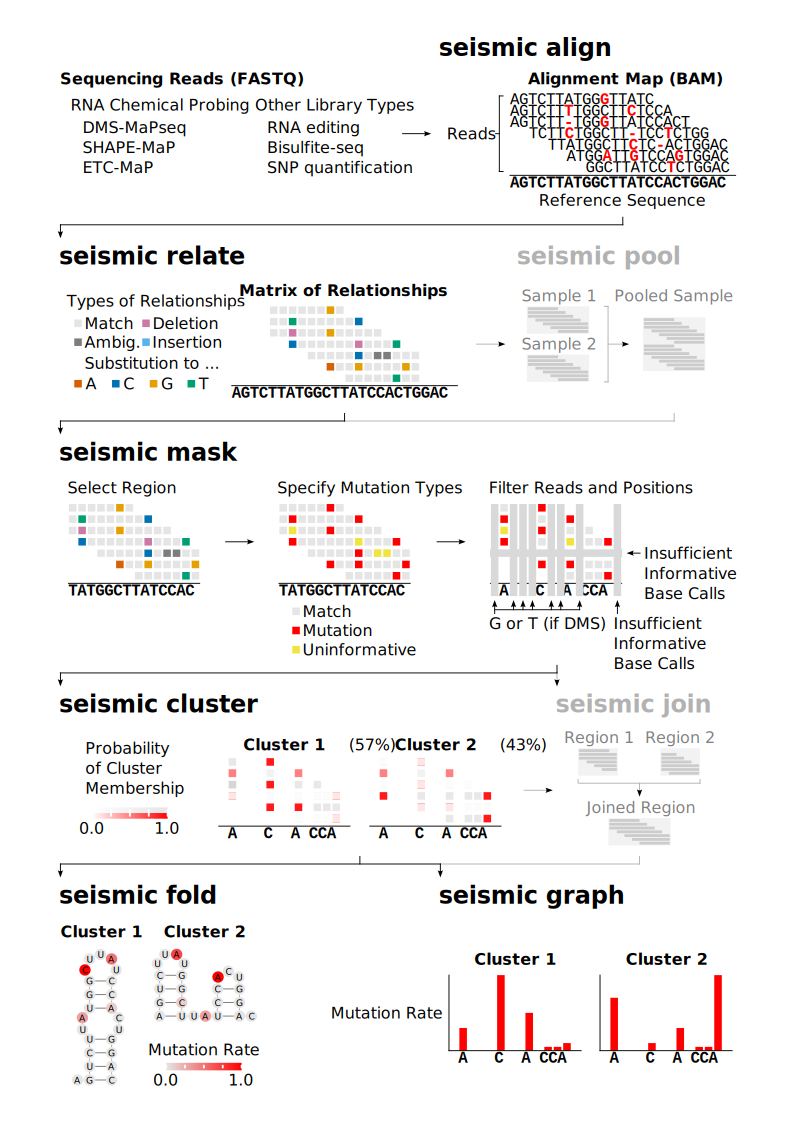
\includegraphics[width=0.95\textwidth]{Figure_1.pdf}
	\caption{\textbf{SEISMIC-RNA processes sequencing reads into predicted RNA structures.} (Continued on next page.)}
	\label{wf}
\end{figure*}
\addtocounter{figure}{-1}
\pagebreak
\begin{figure*}[!t]
	\caption[]{(Continued from previous page.) As input, SEISMIC-RNA accepts sequencing reads from RNA mutational profiling experiments (e.g. DMS-MaPseq~\cite{Zubradt2016} , SHAPE-MaP~\cite{Siegfried2014}, ETC-MaP~\cite{Douds2024}) or other experiments whose readouts are point mutations. SEISMIC-RNA first aligns the reads to the reference sequence of each RNA using Bowtie~2~\cite{Langmead2012}. Next, it determines the relationship (i.e. match, substitution, deletion, insertion) between each read and each position in the reference. It marks low-quality base calls and deletions/insertions in repetitive sequences as ambiguous. It also clips 4 bases from both ends of each read to correct bias against mutations during local alignment. Optionally, users can then pool together multiple samples, such as replicates. Next, SEISMIC-RNA selects relevant data and masks out the remainder: users optionally select a region of the RNA to analyze, specify which relationships to count as mutations, and filter out unusable reads and positions. SEISMIC-RNA then clusters the remaining data to detect alternative RNA structures. Every read is assigned a probability of belonging to each cluster; for each cluster, its proportion is the average of all read probabilities, and its mutation rates are the probability-weighted averages over all reads. Optionally, users can join multiple regions that were masked or clustered individually. SEISMIC-RNA can then use the mutation rates to predict the RNA structure corresponding to each cluster using RNAstructure~\cite{Reuter2010}, as well as generate 13 types of graphs, such as bar graphs of the mutation rates. This entire workflow (except pool and join) can be run with one command: ``seismic wf".}
\end{figure*}
\pagebreak


\begin{figure*}[!t]
    \centering
	\includegraphics[width=0.95\textwidth]{Figure_2.pdf}
	\caption{\textbf{Reads with nearby mutations are underrepresented, producing false clusters unless corrected for.} (Continued on next page.)}
	\label{mutation-gap}
\end{figure*}
\addtocounter{figure}{-1}
\pagebreak
\begin{figure*}[!t]
	\caption[]{(Continued from previous page.) \textbf{(A)} Reads whose two closest mutations have a gap less than 4~nt are underrepresented in DMS-MaPseq data~\cite{Morandi2021} compared to the theoretical expectation if mutations occurred independently. \textbf{(B)} Underrepresentation of reads with nearby mutations can cause false clusters. For an RNA that forms a single structure, reads with two mutations less than 4~nt apart will occur rarely in sequencing data. Thus, the two mutations will be anti-correlated, so a naive clustering algorithm will falsely create a cluster for each mutation. \textbf{(C)} We simulated DMS-MaPseq data for 60 random RNA sequences, each with one true cluster, to have bias similar to that of empirical data. Each light trace represents one simulated dataset; the dark traces are the average of all simulated datasets. \textbf{(D)} Without correcting for the bias in mutation gaps, 95\% of simulated datasets incorrectly yielded more than one cluster. With SEISMIC-RNA's bias correction algorithm, all datasets correctly yielded one cluster. \textbf{(E)} In a representative RNA that yielded two clusters without bias correction, position 83 (red) is one of the most frequently mutated positions and is surrounded by six other positions with mutation rates of at least 2\% (orange). Clustering without bias correction assigned reads in which position 83 was mutated predominantly to cluster 2, and reads in which any surrounding position was mutated predominantly to cluster 1, in agreement with panel (B).}
\end{figure*}

\begin{figure*}[!t]
    \centering
	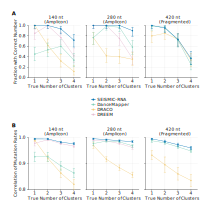
\includegraphics[width=0.95\textwidth]{Figure_3.pdf}
	\caption{\textbf{SEISMIC-RNA is more accurate than similar software.} \textbf{(A)} The fraction of 60 simulations for which SEISMIC-RNA, DanceMapper, DRACO, and DREEM detected the correct number of clusters for each length of RNA and true number of clusters. Error bars show 95\% confidence intervals. \textbf{(B)} The average Pearson correlation between the true mutation rates and those calculated by SEISMIC-RNA, DanceMapper, DRACO, and DREEM for each length of RNA and true number of clusters. Error bars show 95\% confidence intervals.}
	\label{accuracy}
\end{figure*}

\begin{figure*}[!t]
    \centering
	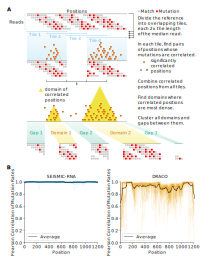
\includegraphics[width=0.95\textwidth]{Figure_4.pdf}
	\caption{\textbf{SEISMIC-RNA clusters long transcripts by first identifying domains that form multiple clusters.} \textbf{(A)} First, SEISMIC-RNA divides a long transcript into tiles, each twice the median read length and overlapping half of each adjacent tile. Within each tile, it finds pairs of positions whose mutations correlate significantly using a hypergeometric test with the Benjamini-Hochberg correction. It then combines correlated pairs from all tiles and identifies domains where pairs are most dense. Finally, it clusters each domain, and optionally each gap between domains. \textbf{(B)} The rolling Pearson correlation (45~nt window size) between the true mutation rates and detected mutation rates for each of the 60 simulated RNAs analyzed with SEISMIC-RNA (transparent blue) or DRACO (transparent orange). The black line shows the average correlation among all simulations.}
	\label{ensembles}
\end{figure*}

\begin{figure*}[!t]
    \centering
	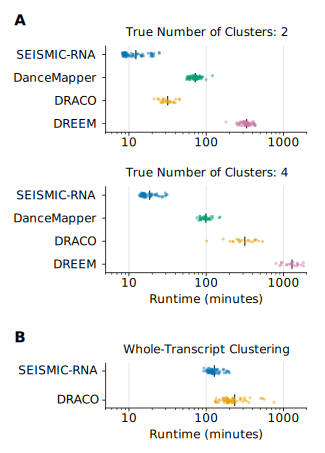
\includegraphics[width=0.5\textwidth]{Figure_5.pdf}
	\caption{\textbf{SEISMIC-RNA is faster than similar software.} \textbf{(A)} Points show the runtime for every simulated dataset of a 280~nt RNA sequence with 200,000 reads whose analysis yielded the true number of clusters. Vertical black bars indicate mean runtimes. For consistency, runtimes of DanceMapper and DRACO include preprocessing with ShapeMapper~2 and RNA Framework, respectively. \textbf{(B)} Similar to (A), but comparing the speed of whole-transcript clustering for the 1,200~nt RNAs.}
	\label{speed}
\end{figure*}


\end{document}
